%!TEX program = xelatex
% 完整编译方法 1 pdflatex -> bibtex -> pdflatex -> pdflatex
% 完整编译方法 2: xelatex -> bibtex -> xelatex -> xelatex
\documentclass[lang=cn,11pt]{elegantpaper}
\usepackage{url}
\usepackage{booktabs}
\usepackage{multirow}
\usepackage{geometry}
\usepackage{longtable}
\usepackage{pdfpages}
\title{基于卷积神经网络和迁移学习的图像识别模型}

% 不需要版本信息, 直接注释即可
% \version{0.07}
% 不需要时间信息的话, 需要把 \today 删除. 
\date{}


% 如果想修改参考文献样式, 请把这行注释掉
% \usepackage[authoryear]{gbt7714}  % 国标

\begin{document}


\newpage
\maketitle

\vspace{-25pt}
\begin{abstract}



\end{abstract}
\keywords{}
	
\tableofcontents
\thispagestyle{empty}
\newpage
\normalsize
\pagenumbering{arabic}


\section{模型实践与改进}

我们使用了sklearn中ensemble类里的AdaBoostClassifier类. 数据集选用了UCI数据集中的IRIS数据集. IRIS数据集是一个花卉分类数据集, 其中给出了标记好的三种花卉(Iris Setosa-山鸢尾, Iris Versicolour-杂色鸢尾, 以及Iris Virginica-维吉尼亚鸢尾), 以及其所对应的四个特征(花萼长度, 花萼宽度, 花瓣长度, 花瓣宽度). 我们的任务是学习一个函数, 使得其通过输入这三种花其中的某一种的一个植株的这四个参数, 能够判断出这个植株是哪一种花. 这是一个典型的分类问题, IRIS数据集也是应用广泛的数据分类数据集. 我们首先将数据集分为训练集与测试集两部分进行训练.

\begin{figure}[hbt]
\centering
  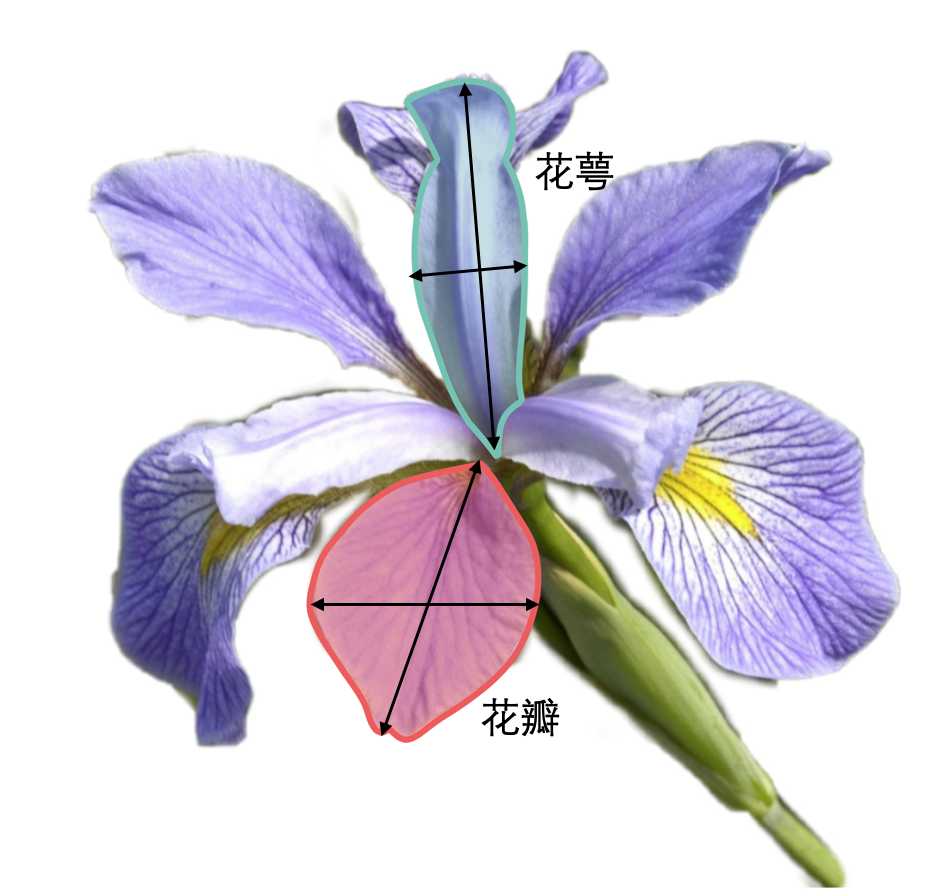
\includegraphics[width=0.75\textwidth]{flower.png}
  \caption{弗吉尼亚莺尾的花萼与花瓣示意图\label{fig:VGflower}}
\end{figure}


\subsection{决策树弱学习机}

我们的模型采用了50个决策树作为弱学习机, 采用了默认的学习率1. Sklearn的AdaboostClassifier能够全自动地帮我们完成优化损失函数%\todo{损失函数是啥}. 
我们在测试集上获得了
的准确率. 


我们还尝试可视化了我们模型的分类边界. 不过由于四维的数据可视化起来比较困难. 我们右只在其中的两个特征上使用相同的方法与参数训练出来了一个学习机, 虽然在性能上有着不小的损失, 准确率从掉到了

, 不过我们觉得很好地解释了我们习得的分类器. 从图上也可以看出这两个特征可以很好的将A类与B、C类分开, 但是对于B、C类之间的分类做的很差. 除了这两个特征我们需要更多的信息去区分B、C类. 

--------------!!!!!BC是哪两类, 特征你用的啥?? 第二个图你解释一下


\subsection{学习机数量提升}

%\todo{改个参数}

那么一个最简单的改进的思路就是去增加弱学习机的数量, 通过更大的学习规模去对函数做更好的拟合. 




我们采用了相同的可视化方案, 重新构建了一个学习机利用两个特征进行分类. 我们的得到的可视化结果与上一次基本上相同, 边的位置有了调整. 意味着增大我们的学习规模虽然可以在一定程度上提升我们分类的准确性, 找到更好的分类边界, 但是其并没有改变分类边界是直线这一致命缺陷, 导致了我们的分类结果的提升非常有限.

\subsection{支撑向量机弱学习机}

由于Boosting过程的特性, 另外一个显然的想法就是尝试不同的弱学习机去提升我们的分类准确率. 我们又尝试了支撑向量机作为我们的弱学习机去进行Adaboosting学习. sklearn.svm类中的svc类给我们提供这样现成的弱学习机. 在支撑向量机里, 我们采用了线性的核函数. 通过使用相同的参数, 我们发现这样的弱学习机的选取也可以极大程度上的影响我们的分类准确率. 我们的分类准确率从%\todo{提升}

提升到了

依旧我们对于两个特征又训练了一个模型用于可视化, 其准确率从

并且可以从图上观察出我们的分类器的确能够相比采用决策树时更好地捕捉到类边界. 相比于决策树的边界而言, SVM作为弱学习机习得的边界不再是一条直线, 故显著增加了分类准确性. 我们还可以观察到在A类与B、C类的分离时几乎没有错分, 但是我们依旧需要更多的信息去区分B、C类.



\newpage
\nocite{*}

% 如果想修改参考文献样式( 非国标 ), 请把下行取消注释, 并换成合适的样式( 比如 unsrt, plain 样式 ). 
\bibliographystyle{unsrt}
\bibliography{wpref}

\end{document}
